\documentclass{exam}
\usepackage{amssymb}
\usepackage{lipsum} 
\usepackage{graphicx}
\usepackage[
backend=biber
]{biblatex}
\addbibresource{refs.bib}

\newcommand\labnr{2}
\newcommand\lab{Lab \labnr\ - Doubly Linked Lists}

\newcommand\uni{Technical University of Cluj-Napoca}
\newcommand\course{Data Structures \& Algorithms}

\newcommand\lvlez{$\bigstar$}
\newcommand\lvlmed{\lvlez\lvlez}
\newcommand\lvlhard{\lvlmed\lvlez}
\newcommand\lvlvhard{\lvlhard\lvlez}


\pagestyle{headandfoot}
\firstpageheader{}{}{}
\firstpagefootrule
\firstpageheadrule
\firstpagefooter{\sc\uni}{}{\sc\course, Lab \labnr}
\runningheader{\sc\uni}{}{\sc\course, Lab \labnr}
\runningheadrule
\runningfootrule
\runningfooter{}{\thepage}{}

\usepackage{listings}
\usepackage{xcolor}
\usepackage{svg}

\definecolor{codegreen}{rgb}{0,0.6,0}
\definecolor{codegray}{rgb}{0.5,0.5,0.5}
\definecolor{codepurple}{rgb}{0.58,0,0.82}
\definecolor{backcolour}{rgb}{0.95,0.95,0.92}

\lstdefinestyle{mystyle}{
    commentstyle=\color{codegreen},
    keywordstyle=\color{magenta},
    stringstyle=\color{codepurple},
    basicstyle=\ttfamily\footnotesize,
    breakatwhitespace=false,         
    breaklines=true,                 
    captionpos=b,                    
    keepspaces=true,                 
    showspaces=false,                
    showstringspaces=false,
    showtabs=false,                  
    tabsize=2
}
\lstset{style=mystyle}

\begin{document}
\begin{center}
    \vspace*{0cm}
    \bfseries\LARGE
    \lab
    \vspace*{1cm}
\end{center}

\section{Doubly linked list}

\noindent Implement a doubly linked list using a structure similar to the following example:

\begin{lstlisting}[language=C]
typedef struct _NODE{
    int key;
    struct _NODE* next;
    struct _NODE* prev;
} NODE;

typedef struct {
    NODE* first;
    // pointer to last node is optional
    NODE* last;
} DLL;
\end{lstlisting}
\includesvg{diagrams/dll.svg}

\bigskip
\noindent Implement a function for each of the following operations:

\begin{questions}
\question List initialisation (create an empty list) \lvlez
\question Insert first \lvlez
\question Delete first \lvlez
\question Insert last \lvlez
\question Delete last \lvlez
\question Get the number of elements in the list \lvlez
\question List deinitialisation (free the memory allocated for the nodes and the list) \lvlez
\question Search element by key. If the element is found return a pointer to the node, otherwise return 0. \lvlmed
\question Delete element by key. If an element with the given key is found in the list delete it. \lvlmed
\question Delete node at arbitrary index. (E.g.: remove the 5th node) \lvlmed
\question Concatenate 2 lists \lvlmed
\question Sort the list \lvlmed
\question Insert node based on an ordering rule (E.g.: node with key 3 will be placed after nodes 1, 2 and before nodes 4, 5) \lvlmed
\question Reverse list \lvlhard
\question Merge 2 ordered lists into a single ordered list \lvlhard
\question Reverse the list without allocating any additional memory. \lvlvhard
\end{questions}

\section{Circular linked list}

\noindent Implement a circular linked list using a structure similar to the following example:

\begin{lstlisting}[language=C]
typedef struct _NODE{
    int key;
    struct _NODE* next;
} NODE;

typedef struct {
    NODE* first;
    // pointer to last node is optional
    NODE* last;
} CLL;
\end{lstlisting}
\includesvg{diagrams/cll.svg}

\bigskip
\noindent Implement a function for each of the following operations:
\begin{questions}
\question List initialisation (create an empty list) \lvlez
\question Insert first \lvlez
\question Delete first \lvlez
\question Insert last \lvlez
\question Delete last \lvlez
\question List deinitialisation (free the memory allocated for the nodes and the list) \lvlez
\end{questions}

\section{Xor doubly linked list}

\noindent Implement a xor doubly linked list using a structure similar to the following example:
\bigskip
\begin{lstlisting}[language=C]
typedef struct _NODE{
    int key;
    size_t both;
} NODE;

typedef struct {
    NODE* first;
    // pointer to last node is optional
    NODE* last;
} XOR_DLL;
\end{lstlisting}

\begin{center}
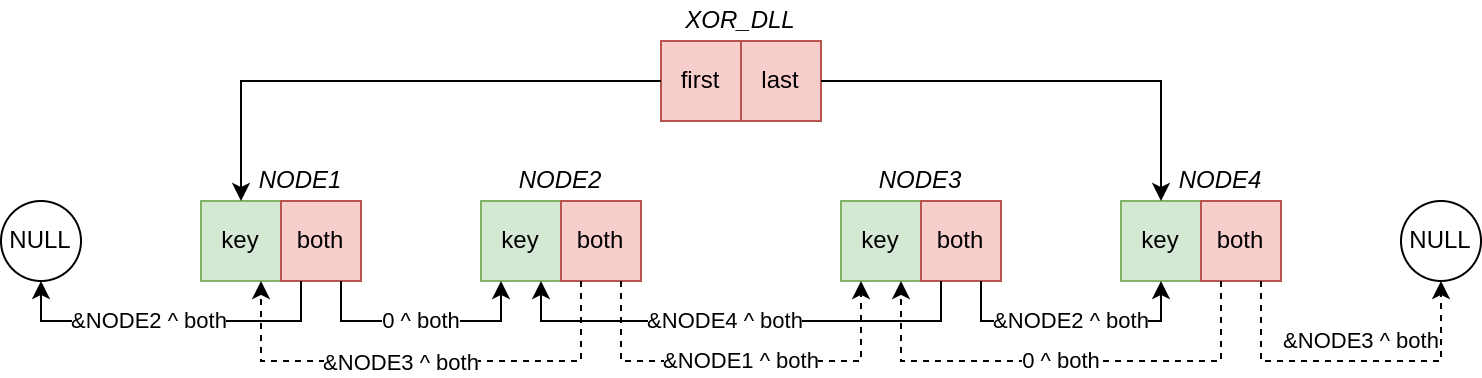
\includegraphics[width=\textwidth]{diagrams/xordll.png}
\end{center}

\bigskip
\noindent Implement a function for each of the following operations:
\begin{questions}
\question List initialisation (create an empty list) \lvlez
\question Insert first \lvlez
\question Delete first \lvlez
\question Insert last \lvlez
\question Delete last \lvlez
\question List deinitialisation (free the memory allocated for the nodes and the list) \lvlez
\end{questions}


\bigskip
\noindent\textbf{Hard mode}: Solve the lab problems using the containing record trick:
\begin{lstlisting}[language=C]
#define CONTAINING_RECORD(address, type, field) (\
    (type *)((char*)(address) - (size_t)(&((type *)0)->field)))
\end{lstlisting}
\textbf{Note:} Leave a comment with the text PB1, PB2, ... PB10 above every function that implements the respective lab task. (upper case text, no space between the text and the problem number)

\medskip
\printbibliography
\end{document}
